%!TEX root = ../hutbthesis_main.tex

\chapter{系统详细设计与实现}

\section{开发与运行环境}

系统的开发，调试，检测和运行都在统一环境下执行，其软硬件设置见表~\ref{tab:dev-env}。

\begin{table}[H]
\centering
\caption{系统开发与运行环境配置}
\label{tab:dev-env}
\begin{tabularx}{0.96\linewidth}{>{\centering\arraybackslash}p{0.24\linewidth} X}
\toprule
类别 & 详细配置 \\
\midrule
操作系统 & Windows 10/11 64位专业版 \\
Python版本 & 3.10.0及以上 \\
仿真平台 & HUTB/CARLA 0.9.13 \\
引擎平台 & Unreal Engine 4.26/5.0及以上 \\
通信框架 & FastMCP最新稳定版 \\
Web框架 & FastAPI + Uvicorn \\
开发工具 & VS Code、PyCharm、Unreal Editor \\
硬件要求 & Intel Core i7及以上，16GB内存，RTX独立显卡（6GB显存以上） \\
\bottomrule
\end{tabularx}
\end{table}

\section{系统整体框架详细设计}

本系统采取交互层-服务层-执行层的三级框架设计，各层职责明晰，接口标准化，数据流向清楚，具有高可靠性，高扩展性和高易用性，系统整体的功能框架见图~\ref{fig:function-framework}。

\begin{figure}[H]
\centering

\includegraphics[width=8.4cm,keepaspectratio]{images/image11.png}
\caption{系统功能框架图}
\label{fig:function-framework}
\end{figure}

在图~\ref{fig:function-framework}中可以清晰明确，当用户通过语音、文本、Web界面或者AI助手输入相关指令时，这时自然语言解析模块识别用户语言意图并提取相关参数，由
MCP 服务调度模块进行指令校验并路由分发，分别对接HUTB
MCP服务（控制车辆、无人机等，接入HUTB/CARLA仿真平台）与Unreal
MCP服务（操作Actor、蓝图等，对接Unreal编辑器内核）；两个仿真平台的状态与数据由采集模块汇总，再经日志与结果返回模块处理，最终通过
Web 可视化交互界面向用户反馈结果。

\section{功能模块详细设计}

\begin{figure}[H]
\centering

\includegraphics[width=0.95\linewidth,keepaspectratio]{images/image12.png}
\caption{模块结构图}
\label{fig:module-structure}
\end{figure}

如图~\ref{fig:module-structure}所示，该系统主要包括五大功能模块：用户交互模块，MCP服务核心模块，HUTB仿真控制模块，
Unreal编辑器控制模块，部署与启动模块

1. 用户交互模块

用户交互模块是整个系统针对操作人员的统一入口，该模块承担指令输入，格式校验，历史记录查询，结果可视化显示以及系统状态监测等功能，给用户赋予简单，统一且易于操作的入口，此模块给出三种标准化交互方式。

Web控制台界面：提供可视化指令输入框、实时日志滚动面板、仿真状态监控区、常用功能快捷按钮，支持鼠标点选操作；

语音输入模块：支持实时语音采集、降噪处理、语音转文本，自动生成可执行指令；

AI助手交互具备多轮对话交互能力，可以对含糊的意图予以澄清，并自动填补缺少的参数，还能成批执行连续指令，从而加强复杂任务的操作效率。

\begin{figure}[H]
\centering
\begin{minipage}{0.47\linewidth}
  \centering
  
\includegraphics[width=6.14cm,keepaspectratio]{images/image13.png}
  \caption{人形机器人智能助手}
  \label{fig:ai-assistant}
\end{minipage}\hfill
\begin{minipage}{0.47\linewidth}
  \centering
  
\includegraphics[width=6.17cm,keepaspectratio]{images/image14.png}
  \caption{下达连接服务器指令}
  \label{fig:server-connect-command}
\end{minipage}
\end{figure}

如图~\ref{fig:ai-assistant}所示，当启动程序时，会自动弹出人形机器人智能助手也就是AI助手来供用户下达命令，此时如图~\ref{fig:server-connect-command}下达连接服务器要求时，会立即连接Carla。

2. MCP服务核心模块

MCP服务模块属于整个系统的关键调度及逻辑处理单元，承担着指令解读，工具守护，路由分配，上下文保存以及通信维持的任务，它内部存在若干子模块；

工具注册子模块：服务启动时自动扫描、加载并注册所有可用功能工具，形成统一工具库；

路由调度子模块：根据识别出的用户意图，自动将指令分发到对应的功能工具与后台服务；

上下文管理子模块：实时维护仿真场景状态、用户会话信息、历史指令记录，保证交互连续性；

通信子模块：负责建立与管理 TCP
网络连接、数据收发、心跳保活与异常自动重连；

日志与异常子模块负责统一记录系统运行的日志，捕捉各种异常错误，并给出标准化的提示信息。

3. HUTB仿真控制模块

HUTB仿真控制模块可达成对HUTB仿真环境全过程的程序化控制，其给予车辆，无人机，环境，传感器，场景编辑等完备的功能接口，

天气环境子模块：负责气象参数设置、时间切换、光照强度调整、环境效果模拟；

\begin{figure}[H]
\centering
\begin{minipage}{0.47\linewidth}
  \centering
  
\includegraphics[width=6.97cm,keepaspectratio]{images/image15.png}
  \caption{晴天天气}
  \label{fig:sunny-weather}
\end{minipage}\hfill
\begin{minipage}{0.47\linewidth}
  \centering
  
\includegraphics[width=6.90cm,keepaspectratio]{images/image16.png}
  \caption{雨天天气}
  \label{fig:rainy-weather}
\end{minipage}
\end{figure}

如图所示，当连接好Calar服务器时，此时的场景天气默认为如图~\ref{fig:sunny-weather}中的晴天，如果用户想要切换天气可通过图~\ref{fig:server-connect-command}中人形机器人智能助手，下达想要切换天气的命令，便可完成切换，例如，当用户下达``天气设置为雨天''时的命令，此时场景变化为图~\ref{fig:rainy-weather}中的雨天天气，除此之外，还能将天气设置为雾天，大风等甚至能满足更多要求如改变光的照射强度等天气需求，来供用户进行车辆仿真。

车辆控制子模块：负责车辆自动生成、位置与姿态控制、自动驾驶开关、车辆状态实时获取；

\begin{figure}[H]
\centering

\includegraphics[width=10.4cm,keepaspectratio]{images/image17.png}
\caption{生成车辆model3}
\label{fig:model3-vehicle}
\end{figure}

如图~\ref{fig:model3-vehicle}所示，通过给AI下达命令``生成车辆model3''时，此时，场景中会生成车辆model3，若用户想要其他车辆，也可将model3改为a2，mustang等其他品牌的车辆，但想要清空车辆，此时只需要下达``清空场景''的命令，车辆便能清除。

\begin{figure}[H]
\centering
\begin{minipage}{0.47\linewidth}
  \centering
  
\includegraphics[width=6.77cm,keepaspectratio]{images/image18.png}
  \caption{车在雨中自动驾驶}
  \label{fig:rain-autodrive}
\end{minipage}\hfill
\begin{minipage}{0.47\linewidth}
  \centering
  
\includegraphics[width=6.38cm,keepaspectratio]{images/image19.png}
  \caption{车辆在雾天自动驾驶}
  \label{fig:fog-autodrive}
\end{minipage}
\end{figure}

生成车辆后，用户便可以再下达，车辆``自动驾驶''时的命令，此时，车辆便会按照路线所建造来自动行驶，还能将车辆与天气系统结合起来，在自动驾驶的过程中，下达改变天气的命令，就能像图~\ref{fig:rain-autodrive}和图~\ref{fig:fog-autodrive}所示的雨天和雾天天气中行驶，当然可以变换更多用户需要的天气来观察记录车辆的行驶，此时不同天气所对车辆造成的不同情况能更还原现实生活所求。若用户需要手动驾驶车辆，也可通过外接手柄等设备，亲身体验车辆驾驶。

\begin{figure}[H]
\centering
\begin{minipage}{0.47\linewidth}
  \centering
  
\includegraphics[width=6.2cm,keepaspectratio]{images/image20.png}
\end{minipage}\hfill
\begin{minipage}{0.47\linewidth}
  \centering
  
\includegraphics[width=6.2cm,keepaspectratio]{images/image20.png}
\end{minipage}
\caption{车辆自动驾驶时状态与场景交通灯状况}
\label{fig:vehicle-status-traffic}
\end{figure}

当用户需要了解此时此刻的场景状态时，下达``获取车辆状态''，AI助手便能快速的获取当下场景时的状态，如图~\ref{fig:vehicle-status-traffic}所示，此时车辆为model3，正在自动驾驶中，车速为28.01km/h，并获取车辆在场景中的地址，当然，以为场景为城市，交通灯也是必不可少的内容，当用户下达``获取交通灯状态''的命令时，AI助手便能实时播报场景之中5个交通灯的状态。如图~\ref{fig:fog-autodrive}所示，5个交通灯中3个为红灯，2个为绿灯。当然如果用户想要主动改变交通灯状况时，便可下达``交通灯全为红灯''或``交通灯全为绿灯''的命令，此时场景中交通状态要么车辆如图~\ref{fig:traffic-red-all}全在灯红灯，要么车辆在城市中畅通无阻。

\begin{figure}[H]
\centering
\begin{minipage}{0.43\linewidth}\centering
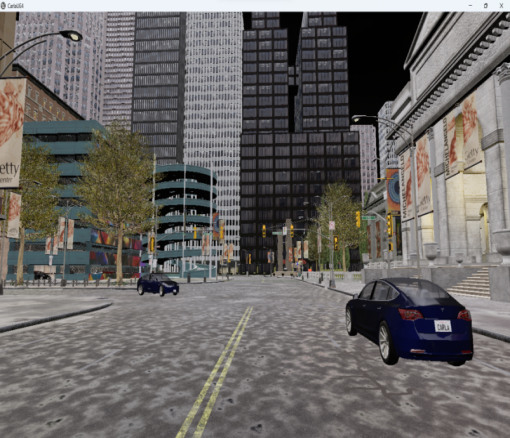
\includegraphics[width=6.2cm,keepaspectratio]{images/image21.png}
\end{minipage}\hspace{0.9cm}
\begin{minipage}{0.43\linewidth}\centering
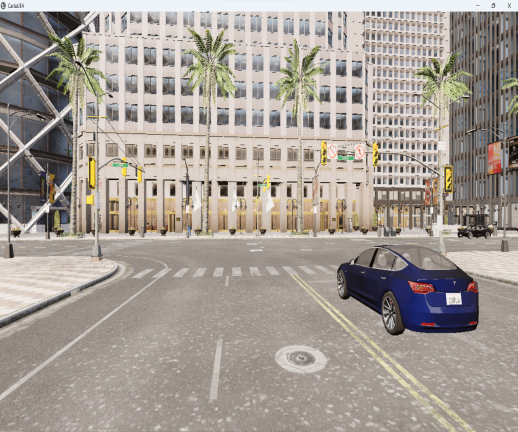
\includegraphics[width=6.2cm,keepaspectratio]{images/image22.png}
\end{minipage}
\vspace{0.6em}

\begin{minipage}{0.43\linewidth}\centering
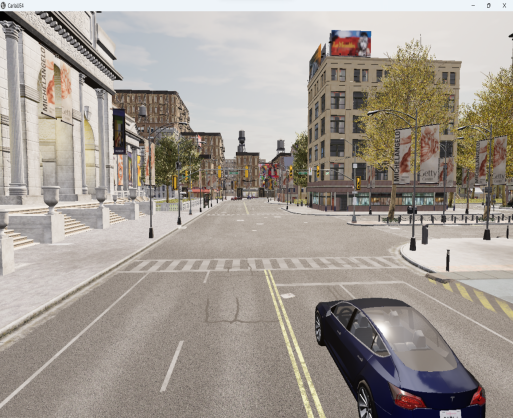
\includegraphics[width=6.2cm,keepaspectratio]{images/image23.png}
\end{minipage}\hspace{0.9cm}
\begin{minipage}{0.43\linewidth}\centering
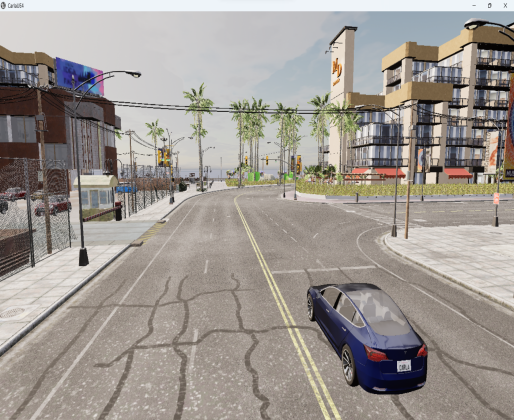
\includegraphics[width=6.2cm,keepaspectratio]{images/image24.png}
\end{minipage}
\vspace{0.6em}

\begin{minipage}{0.43\linewidth}\centering
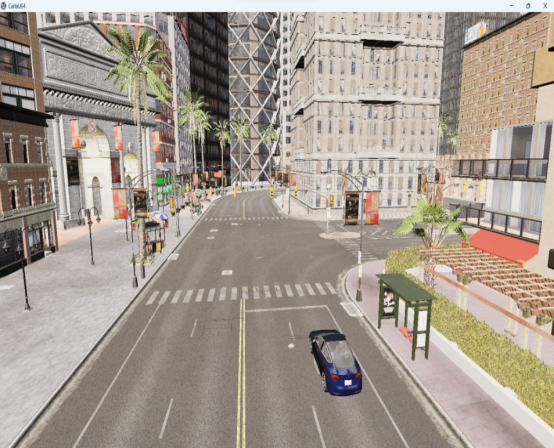
\includegraphics[width=6.2cm,keepaspectratio]{images/image25.png}
\end{minipage}\hspace{0.9cm}
\begin{minipage}{0.43\linewidth}\centering
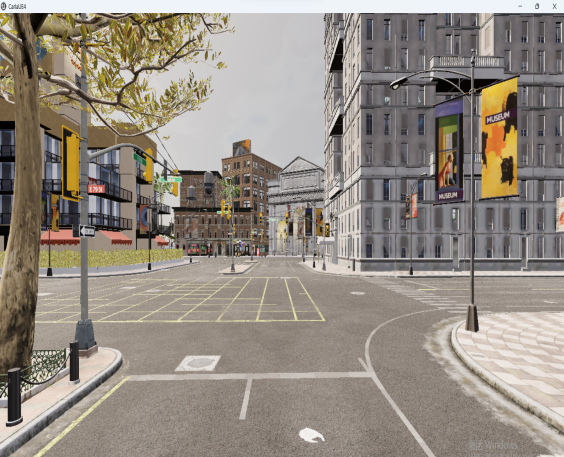
\includegraphics[width=6.2cm,keepaspectratio]{images/image26.png}
\end{minipage}
\caption{交通灯全为红灯}
\label{fig:traffic-red-all}
\end{figure}

4.Unreal编辑器控制模

Unreal编辑器控制模块可对Unreal引擎执行远程程序化控制，做到对场景物体，蓝图，UI，关卡等资源的自动化编辑，

Actor管理子模块：实现场景中物体的添加、删除、修改、查询与属性配置；

蓝图编辑子模块：支持蓝图类创建、逻辑编辑、代码编译与文件保存；

节点图子模块：实现蓝图节点添加、参数配置、节点连线与逻辑执行；

UMG UI子模块：负责界面控件制作、布局排版、事件绑定与交互逻辑设置；

关卡和项目子模块承担着地图加载，项目全局设置以及引擎底层参数设置的任务。

5. 部署与启动模块

部署与启动模块可把整个系统立即，自动化地部署到目标环境当中，不需要人工干预就能完成全过程的设置，自动环境设置，大批量安装依赖库，统一开启后台服务，多进程运作管理，收集运行日志并给出异常提示，从而做到从环境准备到系统启动的全过程自动化，极大地优化了系统的部署效率和稳定性。

\section{核心模块实现}

\subsection{HUTB MCP服务实现}

HUTB
MCP服务属于整个仿真控制系统的关键执行部分，其需同CARLA仿真器形成稳定的关联，并给予标准化的工具接口，该服务的启动过程依照模块化，可设置，可拓展的设计理念来开展。

\begin{figure}[H]
\centering
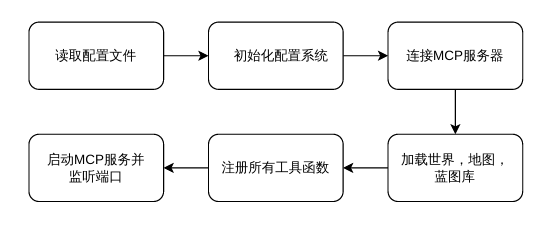
\includegraphics[width=13.3cm,keepaspectratio]{images/image27.png}
\caption{HUTB MCP服务启动流程图}
\label{fig:hutb-mcp-startup}
\end{figure}

如图~\ref{fig:hutb-mcp-startup} HUTB
MCP服务启动流程图所示首先读取外部设置文件，完成端口，路径，日志级别等参数的加载，然后初始化全局日志系统。再经由TCP协议同CARLA服务器创建长连接，执行身份验证和通信握手。连接达成之后加载当下的仿真世界，地图资源，蓝图库以及交通守护者，为后续的实体控制做准备。接着自动扫描并注册全部可用的工具函数，合成统一可调用的工具列表。最后开启MCP服务，进入指令监听状态，等待外部指令下达并执行。

核心代码依托FastMCP框架形成，利用装饰器把普通函数注册成可远程调用的MCP工具，做到接口标准化，参数可校验，返回值结构化，从而让外部系统可以统一调用仿真器的所有功能。

\subsection{Unreal MCP服务实现}

Unreal
MCP服务重点在于同虚幻引擎内部插件开展通信，以达成远程编辑，场景修改，蓝图调用以及资源运作等目的，该服务采取Socket长连接模式，从而与引擎插件维持即时的数据交换，保证指令传送既低延迟又高可靠，在启动期间，服务会自行执行端口绑定，线程初始化，消息队列生成等事务，之后便处于就绪状态，随时等候上层下达的编辑指令。

\begin{figure}[H]
\centering
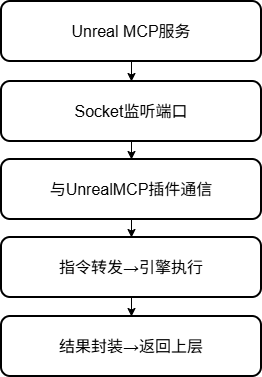
\includegraphics[width=5.5cm,keepaspectratio]{images/image28.png}
\caption{Unreal MCP服务通信架构图}
\label{fig:unreal-mcp-communication}
\end{figure}

如图~\ref{fig:unreal-mcp-communication} Unreal
MCP服务通信架构图所示：UnrealMCP服务收到编辑指令之后，会先对指令执行分析，格式转换以及合法性校验操作，接着把指令传递给虚幻引擎内部去执行，等到执行完毕，服务就能及时得到回传的结果，状态消息和日志数据，然后把这些信息封装成标准格式告知上层模块，这个服务有效地达成了对虚幻引擎的远程程序化操控，使得编辑过程更为自动化，极大地优化了场景创建，资源安排以及调试相关工作的效率。

\subsection{自然语言指令映射实现}

自然语言指令映射是提高系统智能化的重要环节，它可以把用户的口语化、模糊化的要求转化为机器可以理解的标准指令，包括语义理解、关键词提取、意图判别和参数补充等几个方面的工作，以便更好地理解自然语言，在这个过程中，模块会根据上下文对缺失或不清楚的部分进行填充以提高命令识别率。

\begin{figure}[H]
\centering
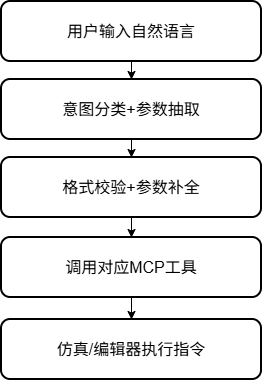
\includegraphics[width=5.2cm,keepaspectratio]{images/image29.png}
\caption{自然语言指令映射执行流程图}
\label{fig:nl-command-execution}
\end{figure}

图~\ref{fig:nl-command-execution}
自然语言指令映射执行流程图，对解析后的指令自动映射到对应的功能接口上，即从自然语言到机器指令的过程，此模块降低用户操作难度，使得不懂专业知识的人也可以轻松完成复杂操作，此外，该模块支持自定义指令规则并可进行扩展，在不断改进识别率基础上使系统更符合实际情况，提高用户体验以及智能化程度。

\subsection{Web可视化界面实现}

Web可视化界面依托轻量化的Web框架而开发，给用户带来简约，直观又易于操作的执行通道，其界面布局采取分区设计，包含指令输入区，日志显示区，状态监测区以及功能控制面板，结构明晰，便于操作，用户可经由界面直接输入自然语言指令，查看即时运行日志，监测仿真状态和服务运行状况，还能执行快速启动，停止，重新开始等操作。

界面采取了响应式布局设计，可以适应不同大小的显示设备，在电脑，平板之类的终端上都会有不错的显示效果，而且，界面具备即时更新数据，提示异常，显示结果和给予状态反馈的功能，这样用户就能清楚地了解系统的运行状况，采用可视化界面之后，整个操作系统变得更为友好，减小了使用的困难程度，改善了工作效能并优化了用户的感受。

\section{一键部署与自动化启动实现}

\subsection{虚拟环境自动配置}

虚拟环境自动配置脚本可以实现在最短时间内搭建起一个开发环境，避免因为版本不对或者缺少依赖导致的问题，在这个脚本中它会检测Python环境然后创建相应的虚拟环境并且一次性把所有需要的依赖都安装好，整个过程不需要手动干预只需要点击开始就可以全部完成，大大降低部署难度。

脚本运行过程中，依次搭建虚拟环境，激活安装依赖，设置路径以及检查环境，以使所有需要的依赖正确加载，在配置成功之后，程序自动输出提示信息给用户，告知其可以进行下一步操作，该自动配置大大简化复杂的环境配置过程，提高效率并且提高了成功概率。

\subsection{一键启动脚本}

一键启动脚本是精简系统启动流程的关键工具，它能依照预先设定的顺序自动开启所有的服务，脚本会逐一启动仿真平台，MCP服务，Web界面这些重要模块，并自行完成关联，初始化以及加载的过程，用户只要轻轻点击一下这个脚本，就可以做到全部的启动动作，不需要自己动手一步步来做。

脚本有错误检测以及状态判断，在某一部分运行失败的情况下，它会弹出相应的提示并且停止后面的步骤以避免错误进一步扩大，一按即用使得整个程序更加简便易上手，尤其是对于一些不懂技术的朋友来说，大大提升了用户体验度。start.bat会自动执行以下操作：检查或者新建虚拟环境，检查或者安装CARLA模块，询问是否启动CARLA服务器，启动Web界面，打开浏览器。

\begin{figure}[H]
\centering
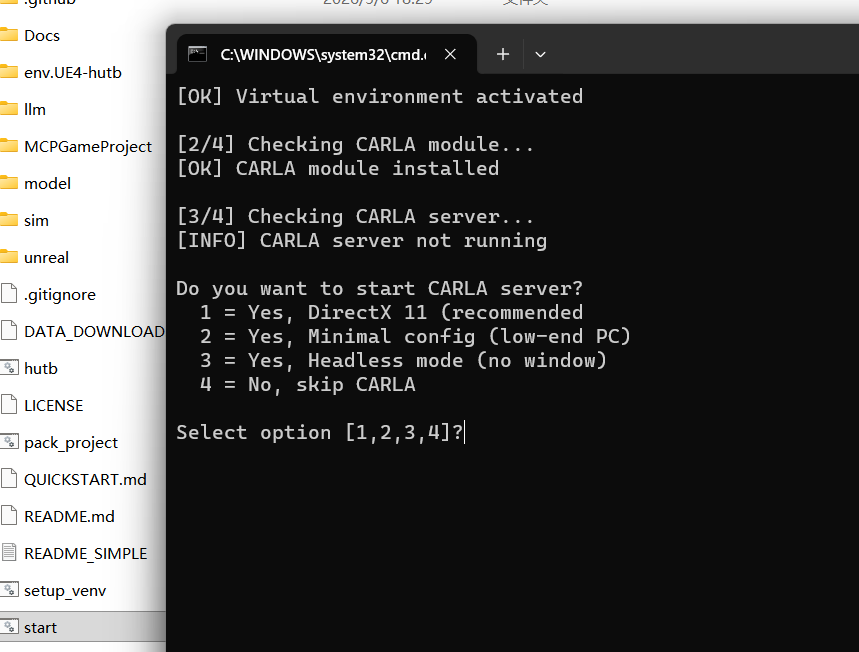
\includegraphics[width=8.6cm,keepaspectratio]{images/image30.png}
\caption{一键启动界面}
\label{fig:one-click-start}
\end{figure}

如图~\ref{fig:one-click-start}所示，当点击``start''后，将会弹出页面，给予用户4中不同选项：

选项1：DirectX11(推荐)适合大多数电脑

选项2：最小配置 适合低端电脑或显存不足

选项3：无头模式 不显示窗口，最省资源

选项4：跳CARLA只使用 AI 对话功能

用户可以根据自身PC的配置情况，选择不同的运行方式，更加适配电脑。



\section{系统运行流程}

整个系统的流程是相当高的自动化水平，在它自启到命令执行的过程中是一个闭合回路，在用户点击运行脚本后，程序就自行进行环境检测、服务初始化、连接建立等工作，随后就处于可以使用的状态，而当用户在网页上输入一条命令之后，这条命令需要被解析、验证、分发等操作，最后才到达对应的功能模块中被执行。

执行完成后，系统会马上把结果返回到界面上，展示日志以及状态等，这一步无需人为干预，十分简单方便而且响应迅速。自动化的运行流程降低了使用难度的同时提高了任务完成的质量与效率，使整个系统更加安全、可靠、易用。

完整流程：首先将文件解压缩后配置好环境，点击start将会弹出图~\ref{fig:one-click-start}的界面，此时用户根据自己电脑配置与需求选择好对应选项。便能同时启动AI人工智能管理系统以及CARLA地图界面如图~\ref{fig:ai-assistant}所示。这时候，用户便可以输入自己的需求给AI，AI便能自动连接好CARLA服务器并等待用户下一步需求。
